% Copyright 2007-2021 Joakim Nilsson
%
% This file is part of Combo Whist.
%
% Combo Whist is free software: you can redistribute it and/or modify
% it under the terms of the GNU General Public License as published by
% the Free Software Foundation, either version 3 of the License, or
% (at your option) any later version.
%
% Combo Whist is distributed in the hope that it will be useful,
% but WITHOUT ANY WARRANTY; without even the implied warranty of
% MERCHANTABILITY or FITNESS FOR A PARTICULAR PURPOSE.  See the
% GNU General Public License for more details.
%
% You should have received a copy of the GNU General Public License
% along with Combo Whist.  If not, see <http://www.gnu.org/licenses/>.

% Document class
\documentclass[a4paper]{article}

\usepackage[swedish]{babel}
% Packages
\usepackage[utf8]{inputenc}
\usepackage{graphicx}              % For \rotatebox
\usepackage{tabularx}              % For the X column specifier
\usepackage[pass]{geometry}        % For changing margins
\usepackage[labelfont=bf]{caption} % Captions boldface
\usepackage{verbatim}
\usepackage{hyperref}

% Set-up reference style
\hypersetup{%
	pdfborderstyle={/S/U/W 1}
}

% Rotate text 90 degrees
\newcommand{\rotccw}[1] {%
	\rotatebox{90}{{#1}}
}

\newcommand{\introPages}{%
	% Title
	\maketitle

	\vfill

	% Logo
	\begin{center}
		\includegraphics[width = \textwidth]{../logo.png}
	\end{center}

	\vfill

	% Copyright 2014-2024 Joakim Nilsson
%
% This file is part of Combo Whist.
%
% Combo Whist is free software: you can redistribute it and/or modify
% it under the terms of the GNU General Public License as published by
% the Free Software Foundation, either version 3 of the License, or
% (at your option) any later version.
%
% Combo Whist is distributed in the hope that it will be useful,
% but WITHOUT ANY WARRANTY; without even the implied warranty of
% MERCHANTABILITY or FITNESS FOR A PARTICULAR PURPOSE.  See the
% GNU General Public License for more details.
%
% You should have received a copy of the GNU General Public License
% along with Combo Whist.  If not, see <http://www.gnu.org/licenses/>.

% License notice
\begin{verbatim}
	Copyright 2007-2024 Joakim Nilsson

	This document is part of Combo Whist.

	Combo Whist is free software: you can redistribute it and/or modify
	it under the terms of the GNU General Public License as published by
	the Free Software Foundation, either version 3 of the License, or
	(at your option) any later version.

	Combo Whist is distributed in the hope that it will be useful,
	but WITHOUT ANY WARRANTY; without even the implied warranty of
	MERCHANTABILITY or FITNESS FOR A PARTICULAR PURPOSE.  See the
	GNU General Public License for more details.
\end{verbatim}
\verb|You should have received a copy of the GNU General Public License|\\
\verb|along with Combo Whist.  If not, see <|\url{http://www.gnu.org/licenses/}\verb|>.|


	\thispagestyle{empty}
	\pagebreak

	% Table of contents and list of tables
	\setcounter{tocdepth}{3}
	\tableofcontents
	\listoftables
	\thispagestyle{empty}
	\pagebreak
}


% Title
\title{\textsc{Kombinations-Whist}}
\author{Av Joakim Nilsson}
\ifdefined\varDev
	\date{Utvecklingsversion (baserad på version \varVersion-\varLanguage)---\today}
\else
	\date{Version \varVersion-\varLanguage\---\today}
\fi

% Document
\begin{document}
	\introPages

	% Links
	\noindent
	\fbox{
		\parbox{\textwidth}{
			För den senaste versionen av reglerna, besök \rulesUrl\ eller följ \rssUrl.
		}
	}

	\pagebreak

	\section{Översikt}
		Kombinations-Whist är ett kortspel som bygger på sticktagande och är---som namnet antyder---en variant av Whist. Kombinations-Whists huvudsakliga utmärkande drag är dess varierade utbud av möjliga strategier med acceptabelt simpla regler. (Det måste dock erkännas att regelboken trots det är någorlunda lång.) Möjligheten att spela enligt många varierade strategier undviker en substantiell mängd slump som vanligtvis finnes i andra Whist-spel utan att att göra spelet alltför komplicerat. Detta gör Kombinations-Whist till ett spel som är kul att spela både för erfarna spelare såväl som för nybörjare.

		\paragraph{Antal spelare:}
		4 är att föredra, men 3 till $\infty$ går också bra med vissa regeljusteringar.

		\paragraph{Vad som behövs för att spela:}
		En standard-kortlek med 52 kort samt penna och papper.

		\paragraph{Kortens rangordning:}
		Från högst till lägst: E, K, D, Kn, 10, 9, 8, 7, 6, 5, 4, 3, 2

	\section{Hur man spelar}
		\subsection{Förberedelser}
			Gör en kolumn för varje spelare på pappret. Detta för att hålla koll på poängställningen samt lite annan information om spelet. Efter att pappret är förberett, slumpa då fram vem som blir giv.

			Om det bara finns 3 spelare, ta ut $\clubsuit 6$, samt alla 7:or, 8:or och 9:or från leken.

		\subsection{Given}
			Det finns två huvudsakliga delar av en giv. Den första är \emph{budgivningen} och den andra är \emph{spelet}. Eftersom det borde bli lättare att förstå dessa två delar i omvänd ordning beskrivs spelet före budgivningen.

			En giv börjar med att given delar ut 13 kort till varje spelare. Därefter börjar budgivningen och när den är avklarad börjar spelet.

			Efter spelet noteras spelarnas poäng och en ny giv börjar där spelaren till vänster om den föregående given blir ny giv.

			\subsubsection{Spelet}
				Spelet spelas likt de flesta Whist-varianter. Spelaren till höger om \emph{spelföraren}\footnote{Begreppet ``spelförare'' förklaras i stycket \textit{\nameref{sec:bidding}}.} börjar med att spela ut ett kort. Sen blir det spelaren till höger om denne som spelar ut nästa kort som dessutom måste följa färg. Därefter spelar näste spelare (till vänster om föregående) ut ännu ett kort som också måste följa det första kortets färg och så vidare till det att alla spelare har spelat ut ett kort vardera.

				Om en spelare har slut kort i den först utspelade färgen får denne saka valfritt kort eller spela en trumf. Till skillnad från många Whist-varianter finns inget trumftvång.

				Den spelare som spelade det högsta kortet i den först utspelade färgen tar hem \emph{sticket} (det vill säga, tar alla utspelade kort och lägger på bordet dem med bildsidan nedåt) såvida ingen har spelat ut en trumf. Om så skulle vara fallet är det den spelare som har spelat ut den högsta trumfen som tar hem sticket. Den spelare som tog hem det senaste sticket spelar ut först i nästa.

			\subsubsection{Budgivningen}
				\label{sec:bidding}
				I Kombimations-Whist budar man med \emph{kombinations-bud}. Ett kombinationsbud består av precis ett standardbud och en valfri mängd (inklusive noll) specialbud. Buden har särskilda tilläggsregler förknippade med dem, vilka appliceras under spelet och poängberäkningen.

				Spelarna budar medsols och spelaren till vänster om given börjar. En spelare kan antingen passa eller buda ett kombinationsbud som är värt mer än föregående kombinationsbud (som vi, från och med nu, helt enkelt kommer att kalla bud). Om en spelare passar är denne ute ur budgivningen och får därför inte göra några nya bud förrän nästa giv. Om alla spelare passar blir det omgiv där samme giv ger igen.

				Ett buds värde definieras som det kombinerade värdet av standard- och specialbudet som det består av. För att ett bud ska få budas måste det ha ett värde av minst 1. Det föreslås att en tidsgräns på 20 sekunder sätts mellan varje bud och 1 minut före det första budet. För nybörjare är dock längre eller inga tidsgränser rekommenderade. Om en spelare inte har lagt ett bud inom den givna tiden så passar denne automatiskt. Budgivningen fortsätter fram till att alla spelare förutom en har passat. Den spelaren blir spelförare och spelet börjar.

				De standardbud och specialbud som finns att tillgå finns listade i Tabellerna~\ref{tab:standardBids}~respektive~\ref{tab:specialBids}. Antalet stick att ta hem för att ett bud ska gå hem finnes i standardbudstabellens ``Stick''-kolumn. Ett specialbud kan inte kombineras med ett annat bud som finns listade i ``Inkompatibilitet''-kolumnen. För övrigt är kombinationsbud som omöjligen kan gå hem oavsett motspelarnas kortfördelning förbjudna. Notera att det finns en skillnad mellan värde och poäng. Värde är budets värde (Rätt gissat!) och poäng är antalet poäng som spelföraren får om dennes bud går hem.

				Om det är oklart \emph{när} en händelse som inträffar på grund av ett bud ska ske, se specialbudens ``Ordning''-kolumn. Ett buds ordning bestämmer i vilken ordning de olika händelserna som ges av dess tillägsregler ska ske. De bud med lägst ordning går först. Alla standardbud har ordningen 0.

			\subsubsection{Poängberäkningen}
				Efter att spelet är klart får spelföraren ett antal poäng baserat på vilket kombinationsbud som lagts och huruvida detta bud gick hem. Om budet gick hem får spelföraren det antal poäng som specificeras ``Poäng''-kolumnen för standardbudet. Om budet inte gick hem så förlorar spelföraren 2 poäng. En spelare kan anta en negativ poängsumma. Om en spelare antar en poängsumma lägre än $-5$, så tillåts denne inte längre att buda i budgivningar. Denne får dock 1 gratispoäng efter varje giv som denne deltar i (även om ingen budar och det blir omgiv).

			\subsubsection{Vem som vinner}
				\label{sec:winning}
				Det finns två varianter av hur man bestämmer vem som vinner i Kombinations-Whist: \emph{klassisk} och \emph{begränsad}.

				\paragraph{Klassisk:}
					Den som först uppnår eller överstiger \emph{vinstsumman} vinner. Vinstsumman börjar på 13, men minskar med 1 varje gång alla spelare har varit giv en gång vardera fram tills dess att vinstsumman går ned till 1. Vinstsumman minskar \emph{efter} att den sista given har spelats och poängen för den given har räknats. En spelare kan endast vinna genom att ett bud går hem och kan därför inte vinna enbart därför att vinstsumman just minskade. En spelare kan inte heller vinna om denne inte har enskilt flest poäng.

				\paragraph{Begränsad:}
					Ett förutbestämt antal bas-rundor spelas (förslagsvis 3), där en runda innefattar att alla spelare har varit giv en gång vardera. När bas-rundorna har spelats vinner näste spelare som går hem med ett bud som resulterar i att denne uppnår enskilt flest poäng. För att förtydliga kan en person vinna i samband med att sista bas-rundan just spelats färdigt.

				\paragraph{Skamvinst} Gemensamt för bägge varianterna gäller att om alla spelare utom en innehar $-5$ poäng eller färre så vinner den spelare som har flest poäng automatiskt. Detta sätt att vinna kallas en \emph{Skamvinst}.

	\section{Övrigt}
		\subsection{Regler för fler än 4 spelare}
			Om fler är 4 spelare deltar i spelet så får alla utom 4 sitta ut (avstå att delta) i varje giv. De spelare som sitter ut är de som sitter närmast till höger om given.
		
		\subsection{Prat}
			En viss mängd av prat tillåts i Kombinations-Whist, men spelarna tillåts inte ge \emph{några som helst} ledtrådar om vad de har för kort.
		
		\subsection{Fusk}
			En spelare som avsiktligen fuskar i Kombinations-Whist får aldrig mer spela spelet eftersom denne uppenbarligen inte respekterar spelets prakt.

	% Bid tables
	\pagebreak
	\newgeometry{left=1cm, right=1cm, top=1cm}
	% Copyright 2007-2021 Joakim Nilsson
%
% This file is part of Combo Whist.
%
% Combo Whist is free software: you can redistribute it and/or modify
% it under the terms of the GNU General Public License as published by
% the Free Software Foundation, either version 3 of the License, or
% (at your option) any later version.
%
% Combo Whist is distributed in the hope that it will be useful,
% but WITHOUT ANY WARRANTY; without even the implied warranty of
% MERCHANTABILITY or FITNESS FOR A PARTICULAR PURPOSE.  See the
% GNU General Public License for more details.
%
% You should have received a copy of the GNU General Public License
% along with Combo Whist.  If not, see <http://www.gnu.org/licenses/>.

\section{Standardbud}
	\begin{center}
		\begin{tabularx}{\textwidth}{
			l
			S[table-number-alignment=center, table-format=1.0]
			S[table-number-alignment=center, table-format=1.0]
			cc|X
		}
				\textbf{Benämning} &
				\rotccw{\textbf{Värde}} &
				\rotccw{\textbf{Poäng}} &
				\rotccw{\textbf{Trumf}} &
				\rotccw{\textbf{Stick}} &
				\textbf{Tilläggsregler}
				\\[-3ex]

				\standardBidItem%
				{Skambud}
				{0}
				{1}
				{nej}
				{varierar}
				{%
					Spelföraren får inte ta hem flest stick---inte ens om nån annan spelare har tagit hem lika många stick.
				}

				\standardBidItem%
				{Trumf}
				{1}
				{1}
				{ja}
				{min 5}
				{%
					Spelföraren bestämmer trumffärg.
				}

				\standardBidItem%
				{Ungefär}
				{1}
				{1}
				{nej}
				{varierar}
				{%
					Före spelets början gissar spelföraren på två möjliga mängder stick denne kommer att ta hem. Spelföraren måste ta hem en av de möjliga mängderna stick som gissades.
				}

				\standardBidItem%
				{Grill}
				{1}
				{2}
				{ja}
				{min 5}
				{%
					Spelföraren börjar med att bestämma trumffärg. Denna trumffärg gäller bara första sticket. Därefter blir den färg som spelades ut i föregångde stick ny trumffärg och så fortsätter det till spelets slut.
				}

				\standardBidItem%
				{Blocktrumf}
				{2}
				{1}
				{ja}
				{min 5}
				{%
					Spelföraren bestämmer trumffärg. Spelföraren får inte spela något trumfkort förrän någon annan splare spelar trumf (såvida inte spelföraren enbart besitter trumfkort).
				}
				
				\standardBidItem%
				{Limbo}
				{2}
				{1}
				{nej}
				{varierar}
				{%
					Spelföraren måste ta hem färre stick av de 7 första sticken än av de 6 sista.
				}
				
				\standardBidItem%
				{Spel}
				{2}
				{2}
				{nej}
				{min 5}
				{%
					---
				}

				\standardBidItem%
				{Exakt}
				{3}
				{2}
				{nej}
				{varierar}
				{%
					Före spelets början gissar spelföraren på en möjlig mängd stick denne kommer att ta hem. Spelföraren måste ta hem den mängd stick som gissades.
				}

				\standardBidItem%
				{Mästarskambud}
				{3}
				{2}
				{nej}
				{varierar}
				{%
					Spelföraren måste ta hem färst stick. Om ingen tar hem färre stick än spelföraren går budet hem.
				}

				\standardBidItem%
				{Maxtrumf}
				{3}
				{3}
				{ja}
				{min 7}
				{%
					Spelföraren väljer trumffärg.
				}

				\standardBidItem%
				{Subtrumf}
				{3}
				{3}
				{ja}
				{min 5}
				{%
					Spelföraren väljer trumffärg. Denne får dock inte välja en trumffärg som denne har flest kort i.
				}

				\standardBidItem%
				{Rangtrumf}
				{3}
				{4}
				{ja}
				{min 5}
				{%
					Alla spelare väljer ett kort var och lägger det på bordet med bildsidan nedåt. Korten vänds sedan upp och spelföraren byter ut sitt kort med det av motspelarnas som är högst. Skulle det finnas flera högsta kort väljer spelföraren ett av dem. Det valda kortets färg är trumffärgen.
				}

				\standardBidItem%
				{Mästarspel}
				{4}
				{3}
				{nej}
				{varierar}
				{%
					Spelföraren måste ta hem enskilt flest stick.
				}

				\standardBidItem%
				{Noll}
				{4}
				{4}
				{nej}
				{0}
				{%
					---
				}

				\standardBidItem%
				{Mästartrumf}
				{6}
				{6}
				{ja}
				{min 5}
				{%
					Spelaren till vänster om spelföraren bestämmer trumffärg, men först får de andra icke-spelförarna säga vilken trumffärg de föredrar och hur mycket de föredrar denna på en skala från 1 till 5 (utan motivering).
				}

				\standardBidItem%
				{Obesudlat Mästarspel}
				{9}
				{*}
				{nej}
				{13}
				{%
					*Om budet går hem får spelföraren lika många poäng som kombinationsbudets värde. Skulle dessutom kombinationsbudets värde vara 13 eller högre vinner spelföraren spelet omedelbart, oavsett poängställning. När detta inträffar erhåller dessutom spelföraren rätten att titulera sig \emph{Obesudlad~Mästare~av~Kombinations-Whist} under resten av sitt liv.
				}
		\end{tabularx}
	\end{center}

	% This file is part of Combo Whist.
%
% Copyright 2007-2019 Joakim Nilsson
%
% This file is part of Combo Whist.
%
% Combo Whist is free software: you can redistribute it and/or modify
% it under the terms of the GNU General Public License as published by
% the Free Software Foundation, either version 3 of the License, or
% (at your option) any later version.
%
% Combo Whist is distributed in the hope that it will be useful,
% but WITHOUT ANY WARRANTY; without even the implied warranty of
% MERCHANTABILITY or FITNESS FOR A PARTICULAR PURPOSE.  See the
% GNU General Public License for more details.
%
% You should have received a copy of the GNU General Public License
% along with this text.  If not, see <http://www.gnu.org/licenses/>.

\newcommand{\nonTrump}{\textnormal{non-trump bids}}

\begin{table}
	\caption{Special bids}\label{tab:specialBids}
	\begin{center}
		\begin{tabularx}{\textwidth}{
			l
			S[table-number-alignment=center, table-figures-decimal=0]
			p{3cm}
			|X
		}
			\textbf{Name} &
			\textbf{Worth} &
			\textbf{Incompatibility} &
			\textbf{Additional rules}
			\\[-3ex]

			\specialBidItem%
			{Triumph Trump}
			{-4}
			{---}
			{%
				The declarer selects any card before the game begins. This card becomes the \emph{triumph trump}. The declarer decides who takes a trick containing the triumph trump when this trick is brought home. A triumph trump does \emph{not} change suit to the trumph suit, but retains its old suit.
			}

			\specialBidItem%
			{Sloth}
			{-3}
			{---}
			{%
				For the tricks in which the declarer doesn't lead, the declarer plays last.
			}

			\specialBidItem%
			{Potential}
			{-2}
			{---}
			{%
				If this bid is completed it is marked by a P, a \emph{potential}, in the declarer's column. The worth of all the declarer's future combo bids increase by \sfrac{1}{2} for each P in the declarer's column.
			}

			\specialBidItem%
			{Start}
			{-2}
			{---}
			{%
				The declarer leads the first trick.
			}

			\specialBidItem%
			{Iron}
			{-1}
			{---}
			{%
				The aces now rank the lowest.
			}

			\specialBidItem%
			{Switcheroo}
			{-1}
			{---}
			{%
				Before the game starts, all players send 3 cards in a direction the declarer chooses (to the right, to the left or across).
			}

			\specialBidItem%
			{Greed}
			{0}
			{---}
			{%
				At the end of the game, one virtual trick is added to or subtracted from the declarer's stick count in such a way that it disfavors them. If the bid is completed, the declarer scores 1 extra point.
			}

			\specialBidItem%
			{Atelier}
			{1}
			{Open~Hand}
			{%
				The declarer chooses 4 cards that they put in \emph{the atelier}. These cards must be shown to all players during the game. As soon as the atelier no longer consists of 4 cards, the declarer must add a card to it, if possible.
			}

			\specialBidItem%
			{Ending Dog}
			{1}
			{Zero}
			{%
				The declarer must not bring home the last trick.
			}

			\specialBidItem%
			{Open Trump}
			{1}
			{\nonTrump, Grill, Open~Hand}
			{%
				The declarer must play with open trump cards. That is, all of the declarer’s trump cards must be shown to all players during the game. If combined with \emph{Atelier}, the atelier must not contain any trump cards.
			}

			\specialBidItem%
			{Lock}
			{2}
			{Zero}
			{%
				The declarer must not bring home any of the first 3 tricks.
			}

			\specialBidItem%
			{Plague}
			{2}
			{Bid~of~Shame, Master's~Bid~of~Shame, Zero}
			{%
				The declarer chooses a suit to be the \emph{plague suit}. The declarer must not become \emph{beplagued}; That is, must not alone bring home the most plague cards (note: \emph{not} tricks), unless they become \emph{honourbly beplagued} and bring home the whole plague suit, in which case they also score an honourable extra point.
			}

			\specialBidItem%
			{Penalty}
			{2}
			{---}
			{%
				If the declarer does not complete their bid, 2 extra points are subtracted from their score.
			}

			\specialBidItem%
			{Master's Switcheroo}
			{3}
			{\nonTrump, Grill}
			{%
				Before the game starts, all players but the declarer sends 4 cards to the player to the right (skipping the declarer). If \emph{Switcheroo} has been bid, the \emph{Switcheroo}-cards are sent before the \emph{Master's Switcheroo}-cards.
			}

			\specialBidItem%
			{Open Hand}
			{3}
			{Atelier, Open~Trump}
			{%
				The declarer must play with an open hand. That is, all of the their cards must be shown to all players during the game.
			}
		\end{tabularx}
	\end{center}
\end{table}

\end{document}
